\documentclass[11pt,a4paper]{moderncv}
\moderncvtheme[blue]{classic}
\usepackage[utf8]{inputenc}
\usepackage[top=1.0cm, bottom=1.0cm, left=1.0cm, right=1.0cm]{geometry}
\usepackage[english]{babel}
\setlength{\hintscolumnwidth}{3.5cm} % width of the left column (dates)
\usepackage{multicol} % multi-columns itemize
%\setlength{\makecvtitlenamewidth}{20cm}

\firstname{Romain}
\familyname{Pellerin}
\title{Principal Engineer at Doctolib GmbH}
%\photo[54pt][0.0pt]{picture} % '64pt' is the height the picture must be resized to, 0.0pt is the thickness of the frame around it (put it to 0pt for no frame) and 'picture' is the name of the picture file
\address{}{\textbf{Open to relocation}}{} % street, city, country
\email{contact@romainpellerin.eu}
\homepage{romainpellerin.eu}
%\mobile{+33 6 95 60 57 81}
\extrainfo{\href{https://github.com/rpellerin}{github.com/rpellerin}}
%\quote{Objective: a full-time job from September 2017}
\renewcommand*{\quotefont}{\Large\bfseries} % override quote's default style
\definecolor{color1}{rgb}{0,0,0} % Overwrites the default blue color

% I took the original code from moderncvstylebanking.sty and changed line 25
% USEFUL for theme banking
% \makeatletter
% \renewcommand*{\maketitle}{%
%   \setlength{\maketitlewidth}{1.0\textwidth}%
%   \hfil%
%   \parbox{\maketitlewidth}{%
%     \centering%
%     % name and title
%     \namestyle{\@firstname~\@lastname}%
%     \ifthenelse{\equal{\@title}{}}{}{\titlestyle{~|~\@title}}\\% \isundefined doesn't work on \@title, as LaTeX itself defines \@title (before it possibly gets redefined by \title)
%     % detailed information
%     \addressfont\color{color2}%
%     \ifthenelse{\isundefined{\@addressstreet}}{}{\addtomaketitle{\addresssymbol\@addressstreet}%
%       \ifthenelse{\equal{\@addresscity}{}}{}{\addtomaketitle[~--~]{\@addresscity}}% if \addresstreet is defined, \addresscity and \addresscountry will always be defined but could be empty
%       \ifthenelse{\equal{\@addresscountry}{}}{}{\addtomaketitle[~--~]{\@addresscountry}}%
%       \flushmaketitle\@firstmaketitleelementtrue\\}%
%     \collectionloop{phones}{% the key holds the phone type (=symbol command prefix), the item holds the number
%       \addtomaketitle{\csname\collectionloopkey phonesymbol\endcsname\collectionloopitem}}%
%     \ifthenelse{\isundefined{\@email}}{}{\addtomaketitle{\emailsymbol\emaillink{\@email}}}%
%     \ifthenelse{\isundefined{\@homepage}}{}{\addtomaketitle{\homepagesymbol\httplink{\@homepage}}}%
%     \collectionloop{socials}{% the key holds the social type (=symbol command prefix), the item holds the link
%       \addtomaketitle{\csname\collectionloopkey socialsymbol\endcsname\collectionloopitem}}%
%     \ifthenelse{\isundefined{\@extrainfo}}{}{\addtomaketitle{\@extrainfo}}%
%     \flushmaketitle}\\[2.5em]}% need to force a \par after this to avoid weird spacing bug at the first section if no blank line is left after \maketitle
%  \makeatother

\begin{document}
\makecvtitle
\vspace{-25pt}
\section{Experience}
\cventry{Oct 2020 -- Present}{Principal Engineer}{\href{https://www.doctolib.de/}{Doctolib GmbH}}{Berlin (Germany)}{}{
\begin{itemize}
    \item Follow-up work with feature teams focused on the pro website: review of technical pre-project planning and documents, pair programming, advise and help with technical debt and legacy code
    \item Cross-team work: large-scale projets synchronization, tasks priorization, various tech initiaves
    \item Scability and risk management: support, mitigation and prevention of down incidents
    \item Interviewing engineering managers and software engineers; mentorship
\end{itemize}~\\
Stack: Ruby on Rails, PostgreSQL, Resque, Redis, ElasticSearch, React. Our CI executes 20,000+ integration tests (Minitest + Capybara) and a few hundred model and unit tests (JavaScript and Ruby).\\\\
Additional relevant keywords: Monolith, AWS, TeamCity, New Relic, Sentry, Jest, SCSS.
}
\vspace{10pt}
\cventry{Jan 2020 -- Oct 2020}{Software Engineer}{\href{https://www.doctolib.de/}{Doctolib GmbH}}{Berlin (Germany)}{}{
\begin{itemize}
    \item Worked on the pro website as a fullstack developer
    \item Helped onboard new joiners and train current employees
    \item Project management in an agile environment (SCRUM-like)
    \item Interviewed engineering managers and software engineers
\end{itemize}
}
\vspace{10pt}
\cventry{Mar 2018 -- Dec 2019}{Software Engineer}{\href{https://www.doctolib.fr/}{Doctolib}}{Paris (France)}{}{Same as in Berlin, different feature team.}
\vspace{10pt}
\cventry{Sep 2017 -- Feb 2018}{Software Engineer}{\href{https://matters.tech/}{Matters}}{Paris (France)}{}{
Worked for a client (\href{https://wisepops.com}{Wisepops.com}) on a web-based popup editor built with React.\\Stack: JavaScript (React, Redux, NodeJS), CSS.
}
\vspace{10pt}
\cventry{Feb 2017 -- Jul 2017}{Software Engineer Intern}{\href{https://matters.tech/}{Matters}}{San Francisco (USA)}{}{
Boostrapped \href{https://teamstarter.co/}{Teamstarter.co}. Also experimented new technologies: asm.js and WebAssembly.\\
Stack: JavaScript (React, Redux, \href{https://sequelizejs.com/}{Sequelize}), \href{https://graphql.org/}{GraphQL}, \href{https://www.apollodata.com/}{Apollo}, PWA (Service Workers).
}
\vspace{10pt}
\cventry{Sep 2015 -- Feb 2016}{Mobile Developer Intern}{\href{http://www.wearesmiths.com/}{The Smiths}}{Amsterdam (The Netherlands)}{}{
\begin{itemize}
    \item iOS/Android development with \href{https://www.appcelerator.com/Titanium/}{Titanium/Alloy (framework)}, Backbone.js, Underscore.js
  \item Back-end development with Express.js, hosted on \href{http://www.parse.com/}{parse.com}. Also some SQL and Shell-scripting.
\end{itemize}}
\vspace{10pt}
\cventry{Jun 2013 -- Sep 2014}{Android and Web Developer}{Self-employed and then intern}{Nantes (France)}{}{Developed and maintained the Android application and the website of the startup \textsc{\href{http://www.who-wanna.com/en/}{WhoWanna}}. Stack: Java, PHP, MySQL, JavaScript, HTML, CSS, Scala.}%\newline{}

\vspace{10pt}
\section{Education}
\cventry{Sep 2014 -- Jul 2017}{Diplôme d'ingénieur en informatique (Software engineering degree)}{\href{https://www.utc.fr/formations-enseignements/genie-informatique.php}{Université de Technologie de Compiègne (UTC)}}{Compiègne (France)}{}{
\begin{multicols}{2}
\begin{itemize}
\item \textbf{LO17} Indexing and search engines
\item \textbf{L021} Object-oriented programming (C++)
\item \textbf{MB11} Revision of mathematics
\item \textbf{MI01} Architecture of a CPU
\item \textbf{NF11} Programming language theory
\item \textbf{NF16} Algorithms and data structures
\item \textbf{NF17} Databases design
\item \textbf{RO03} Combinatorial optimization
\item \textbf{SC12} Technology, cognition, perception
\item \textbf{SI28} Interactive writing and multimedia
\item \textbf{SR02} Operating systems
\item \textbf{SR03} Web application architectures
\item \textbf{SR05} Distributed algorithms and systems
\item \textbf{SY31} Sensors for smart systems
\item \textbf{LA13, LA15, LB14, SI14} English courses
\end{itemize}
\end{multicols}
} % year, degree, institution, city+picture = {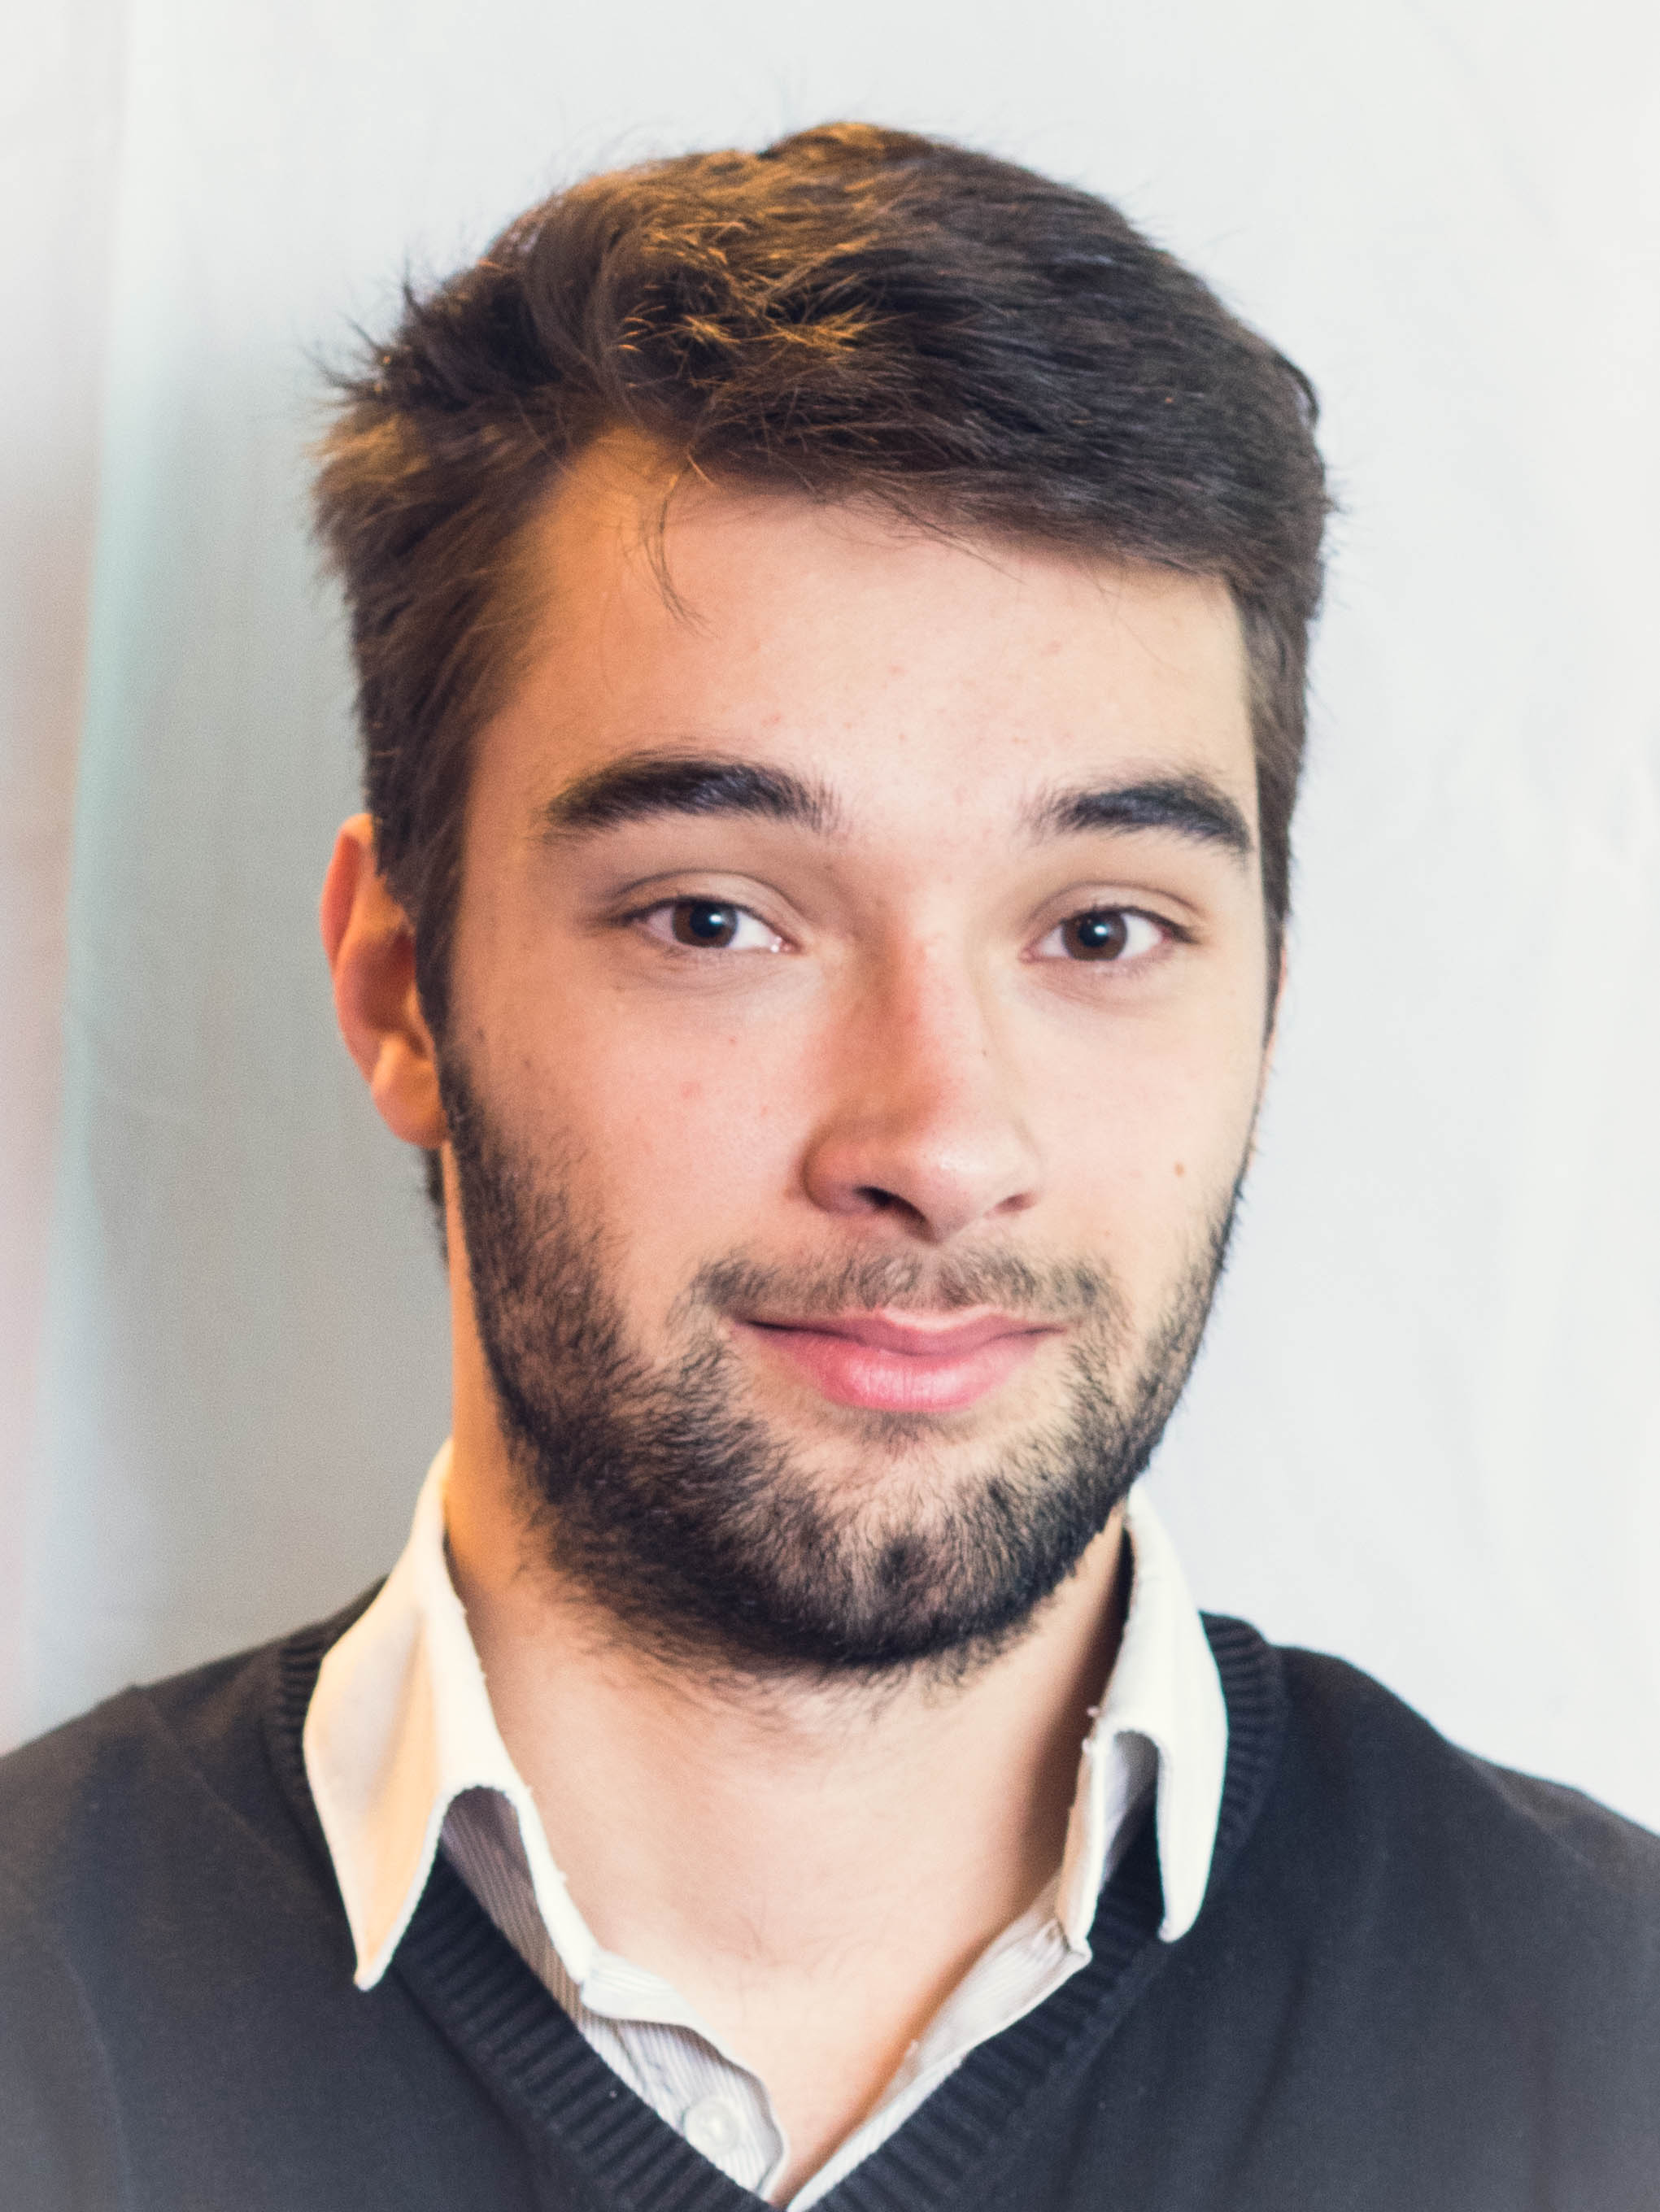
\includegraphics[scale=0.5]{picture}City}, grade, description
\vspace{10pt}
\cventry{Sep 2016 -- Dec 2016}{Exchange program}{\href{https://www.kaist.ac.kr/html/en/}{KAIST}}{Daejeon (South Korea)}{}{
\begin{multicols}{2}
\begin{itemize}
\item \textbf{CS453} Automated Software Testing
\item \textbf{CS459} Introduction to Services Computing
\item \textbf{CS540} Network Architecture
\item \textbf{KSE652} Social Computing Systems Design and Analysis
\end{itemize}
\end{multicols}
} % year, degree, institution, city+picture = {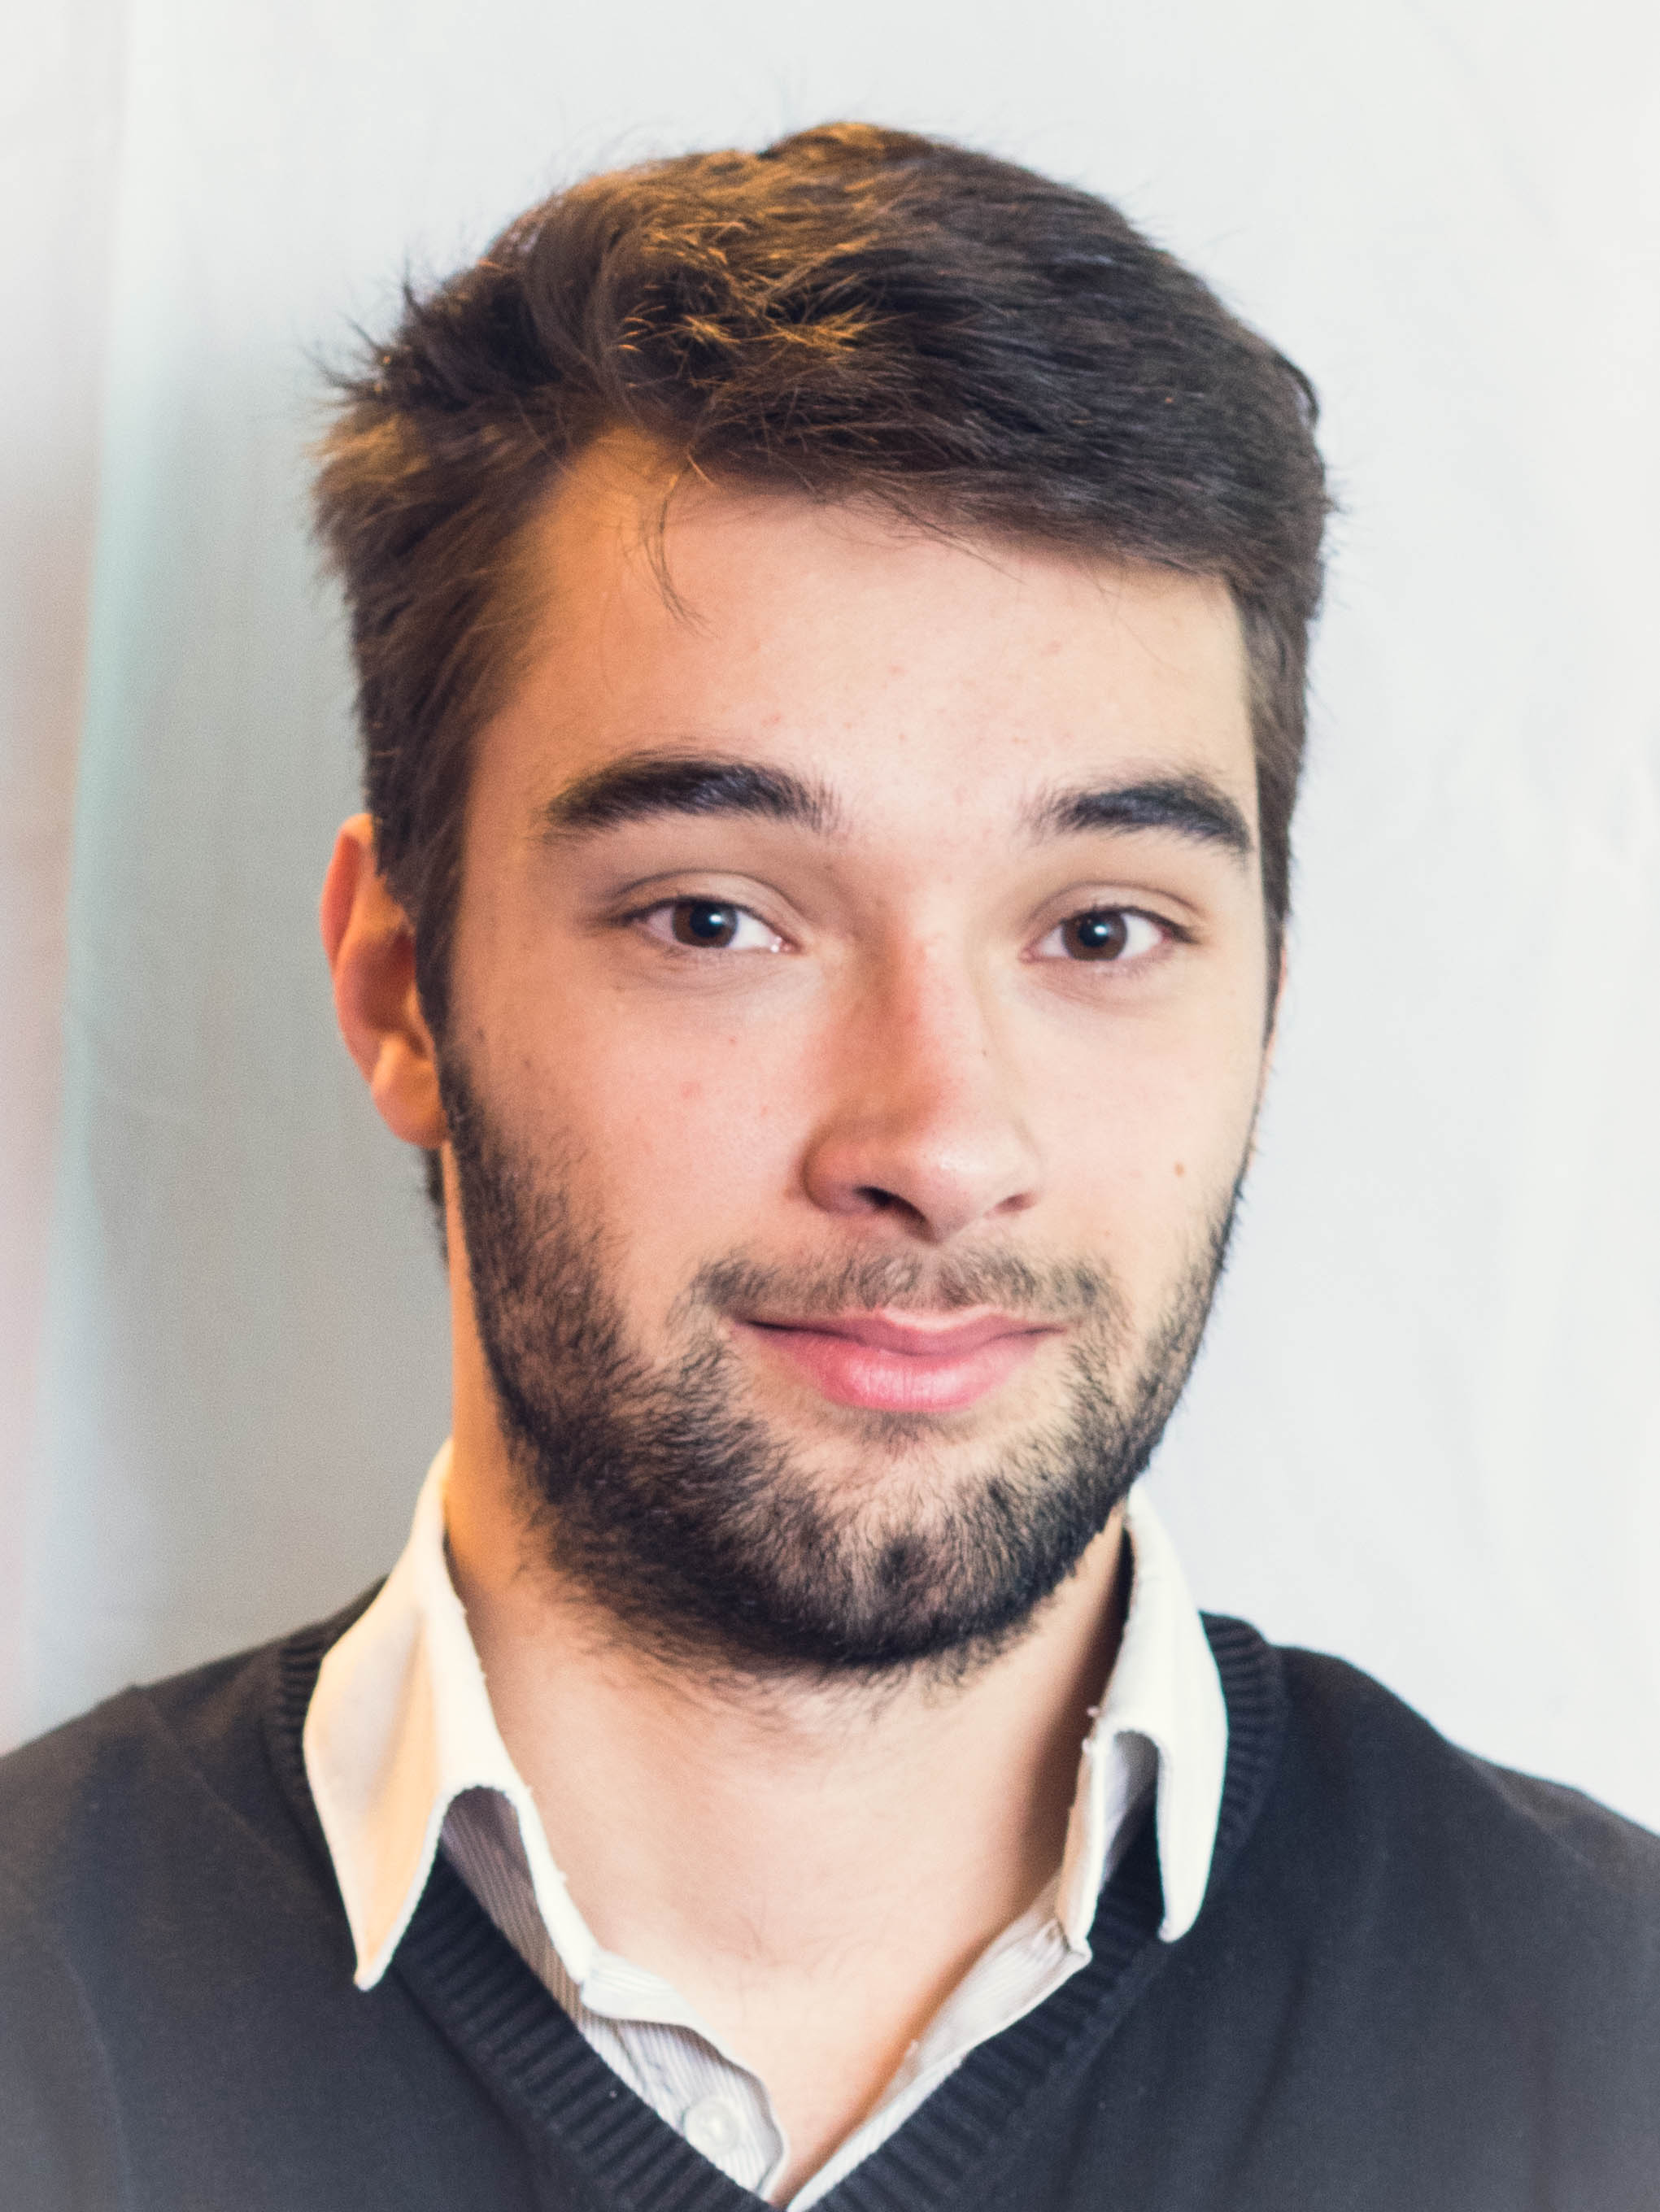
\includegraphics[scale=0.5]{picture}City}, grade, description
\vspace{10pt}
\cventry{Sep 2012 -- Jul 2014}{DUT Informatique (Two-year university degree in Computer Science)}{\href{https://www.iutnantes.univ-nantes.fr/321/0/fiche___formation/}{Institut Universitaire de Technologie de Nantes}}{Nantes (France)}{}{
\begin{multicols}{2}
\begin{itemize}
\item Maths (algebra, set theory, graphs, probability and statistics, automata theory)
\item Systems (Unix, x86 assembly, C, security)
\item Networks (IP/TCP, Wifi and Ethernet, HTTP)
\item Object-oriented programming (Java) and design patterns
\item Web (HTML, CSS, JavaScript, PHP)
\item Databases (Oracle, MySQL)
\item Communication
\item Economy
\item Business management
\item English
\end{itemize}
\end{multicols}
}

\vspace{10pt}
\section{Volunteer Experience}
\cventry{Mar 2015 -- Jun 2015}{President and co-organizer of tech talks}{\href{https://www.youtube.com/playlist?list=PL3nMxbEwNq0wE3BNx5b0EEtp8h-yvHyIy}{HumanTalks}}{Compiègne (France)}{}{10-min talks given once a month about programming languages, tools, software development, etc.\\\href{https://humantalks.com/cities/compiegne}{https://humantalks.com/cities/compiegne}}
\cventry{Sep 2014 -- Jun 2015}{Computer Science Manager}{\href{http://www.usec-utc.fr/}{USEC} (student society)}{Compiègne (France)}{}{Was in charge of software development projects for local businesses.
\begin{itemize}
  \item Wrote official documents (quotes, specifications, customer agreements)
  \item Recruited and mentored students (those who developed our clients' projects)
\end{itemize}}

\vspace{10pt}
\section{Computer Skills}
% \cvcomputer{category}{programs}{category}{programs}
% \cvdoubleitem{subtitle}{text}{subtitle}{text}
\cvitem{Languages}{\textbf{JavaScript, Ruby, HTML, CSS}, Python, PHP, Java, Shell-scripting}
\cvitem{Databases}{\textbf{PostgreSQL, MySQL}, SQLite, UML}
\cvitem{OSes}{\textbf{GNU/Linux} (\href{https://xubuntu.org/}{Xubuntu} user, a Debian/Ubuntu-based distro)}
\cvitem{Misc}{\textbf{React, Ruby on Rails, Git}, NodeJS, \LaTeX}

\vspace{10pt}
\section{Languages}
\cvlanguage{French}{Native speaker}{}
\cvlanguage{English}{Full professional proficiency -- European C2 level}{\textbf{TOEIC 985/990 (March 2016)}}
\cvlanguage{Spanish}{Beginner -- European A2 level}{}
\cvlanguage{German}{Beginner -- European A2 level}{}

\vspace{10pt}
\section{Hobbies}
\cvdoubleitem{\textbf{Raspberry Pi:}}{Websites, VPN, Nextcloud}{\textbf{Side-projects:}}{Android apps, web browser add-ons}
\cvdoubleitem{\textbf{Music:}}{Guitar for fifteen years}{\textbf{Sport:}}{Workout and cycling (3000 kms in 2019)}
\cvdoubleitem{\textbf{Conferences:}}{I gave talks (HumanTalks) and attended some such as \href{https://devfest.gdgnantes.com/}{DevFest}, \href{https://web2day.co/}{Web2Day}, React Europe}{}{}
\end{document}
